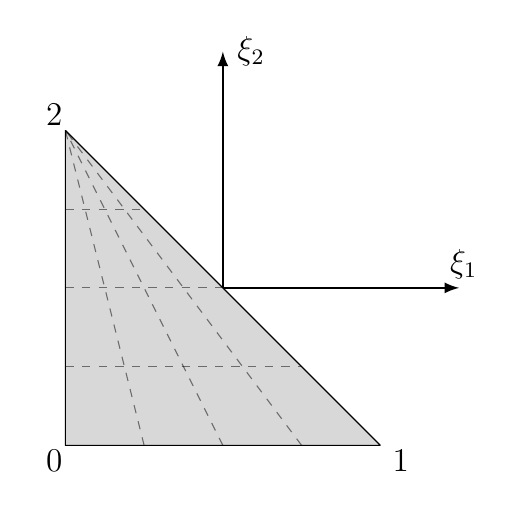
\begin{tikzpicture}[line join=bevel,scale=2,>=latex]
  \coordinate (n0) at (-1,-1);
  \coordinate (n1) at (1,-1);
  \coordinate (n2) at (-1,1);

  \coordinate (n3) at (-0.5, -1);
  \coordinate (n4) at (0, -1);
  \coordinate (n5) at (0.5, -1);

  \coordinate (n6) at (0.5, -0.5);
  \coordinate (n7) at (0, 0);
  \coordinate (n8) at (-0.5, 0.5);

  \coordinate (n9) at (-1, 0.5);
  \coordinate (n10) at (-1, 0);
  \coordinate (n11) at (-1, -0.5);

  \coordinate (C) at (0, 0);
  \coordinate (j) at (0, 1.5);
  \coordinate (i) at (1.5, 0);

  \begin{scope}[blend mode=multiply]
    \fill[black!30,fill opacity=0.5] (n0) -- (n1) -- (n2) -- cycle;
  \end{scope}
  
  \draw (n0) -- (n1) -- (n2) -- cycle;
  \draw[dashed,opacity=0.5] (n3) -- (n2);
  \draw[dashed,opacity=0.5] (n4) -- (n2);
  \draw[dashed,opacity=0.5] (n5) -- (n2);
  \draw[dashed,opacity=0.5] (n11) -- (n6);
  \draw[dashed,opacity=0.5] (n10) -- (n7);
  \draw[dashed,opacity=0.5] (n9) -- (n8);

  \draw[thick, ->] (C) -- (i);
  \draw[thick, ->] (C) -- (j);
  \node at (1.5, 0.15) {\fontsize{12}{12} \selectfont $\xi_1$};
  \node at (0.15, 1.5) {\fontsize{12}{12} \selectfont $\xi_2$};
  \node at (-1.1, -1.1) {\fontsize{12}{12} \selectfont $0$};
  \node at (1.1, -1.1) {\fontsize{12}{12} \selectfont $1$};
  \node at (-1.1, 1.1) {\fontsize{12}{12} \selectfont $2$};
  
\end{tikzpicture}
